\section{Related Approaches}
\begin{frame}{Related Approaches}
  \begin{itemize}
    \item Optimization
      \begin{itemize}
        \item Deterministic
        \item Stochastic
      \end{itemize}
      \vspace*{14pt}
    \item Properties
      \begin{itemize}
        \item Stability
        \item Robustness
      \end{itemize}
      \vspace*{14pt}
    \item Utilizing global information
      \begin{itemize}
        \item Estimation of Distribution Algorithm (EDA)
        \item Model building
      \end{itemize}
  \end{itemize}
\end{frame}

\subsection{Real-coded Extended Compact Genetic Algorithm}


\begin{frame}{Discretization} 
  \begin{itemize} 
    \item Continuous domain $\rightarrow$ Discrete domain 
    \item Finding good solutions $\rightarrow$ Finding promising
      regions
    \item 2 traditional discretization methods
      \begin{itemize}
        \item Fixed-Height Histogram (FHH)
        \item Fixed-Width Histogram (FWH)
      \end{itemize}
      \vspace*{2pt}
  \end{itemize}
  \begin{minipage}{.45\textwidth}
    \begin{figure}
      \centering
      \includegraphics[width =0.5\linewidth]{FHH.eps}
      \caption{Illustration of FHH}
    \end{figure}
  \end{minipage}
  \begin{minipage}{.45\textwidth}
    \begin{figure}
      \centering
      \includegraphics[width =0.5\linewidth]{FWH.eps}
      \caption{Illustration of FWH}
    \end{figure}
  \end{minipage}

\end{frame}

\begin{frame}{Split on Demand}
  \begin{itemize}
    \item Solutions in each bin should not exceed $\gamma N$.
      \begin{itemize}
        \item $N$ is the population size.
        \item $\gamma$ defines the rate of one region.
      \end{itemize}
    \item $\gamma$ decays with a factor $\epsilon$.
  \end{itemize}
  \hspace{-9cm}
  \vspace*{-0.5cm}
  \begin{figure}[h]
    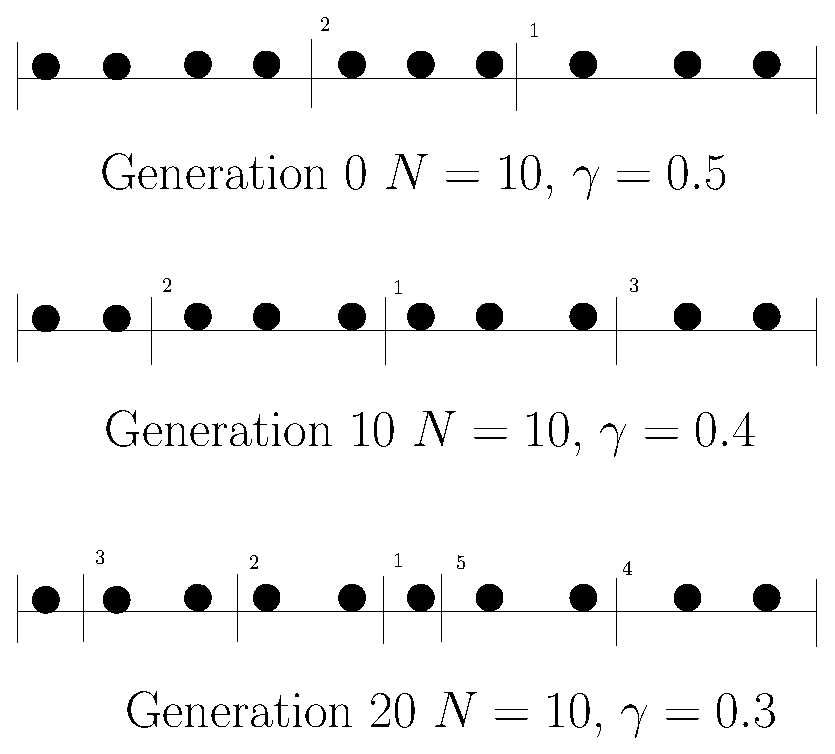
\includegraphics[scale = 0.2]{SoD.eps}
    \caption{Illustration of SoD}
  \end{figure}
\end{frame}

\begin{frame}{EDA}
  \begin{columns}
    \begin{column}{.65\textwidth}
      \begin{itemize}
        \item Sometimes known as Probabilistic Model Building GA (PMBGA).
          \begin{itemize}
            \item Building model explicitly.
            \item Linkage between decision variables are provided.
          \end{itemize}
          \vspace*{14pt}
        \item  Extended Compact Genetic Algorithm (ECGA).
          \begin{itemize}
            \item Model is built according to population distribution.
            \item Applying greedy search to refine model iteratively.
          \end{itemize}
         % \begin{figure}
         %   \centering
         %   \only<4>{\includegraphics[height = 0.5\textheight]{EDA.eps}}
         % \end{figure}
      \end{itemize}
    \end{column}
    \begin{column}{.35\textwidth}
      \begin{figure}[htp]
        \centering
        \includegraphics[width = 0.8\textwidth]{EDA.eps}
        \caption{EDA}
      \end{figure}
    \end{column}
  \end{columns}
\end{frame}

\begin{frame}{Real-coded ECGA with SoD}
  \vspace*{14pt}
  \begin{figure}
    \flushleft
    
    \includegraphics[width=.6\textwidth]{rECGA.eps}
    \caption{rECGA}
  \end{figure}
  %\pause
  %\begin{enumerate}
  %  \item Preparing discretization\pause
  %    \vspace*{14pt}
  %  \item Integrating discretized results into ECGA.\pause
  %    \vspace*{14pt}
  %  \item ECGA builds model accordingly, output the promising
  %    regions.\pause
  %    \vspace*{14pt}
  %  \item Sampling accordingly.\pause
  %    \vspace*{14pt}
  %  \item For every $L$ generations, a local optimizer is adopted to
  %    obtain high resolution solutions\pause
  %    \vspace*{14pt}
  %  \item If model does not converge, goto 1.
  %\end{enumerate}
\end{frame}

\subsection{Covariance Matrix Adaptation Evolution Strategy}


\begin{frame}{Evolution Strategy (ES)}
  \begin{itemize}
    \item A search template for black-box optimization.
      \begin{itemize}
        \item Encoded in continuous domain.
      \end{itemize}
      \vspace*{14pt}
    \item New search points are generated based on current population.
      \vspace*{14pt}
    \item $(\mu,\lambda)$-ES and $(\mu+\lambda)$-ES.
      \vspace*{14pt}
    \item $x_i^{t+1} = m^t + \sigma N_i(0,C)$.
      \begin{itemize}
        \item $x_i^{t+1}$: $i$-th generated solution at generation $t+1$.
        \item $m^t$: weighted mean of population at generation $t$.
        \item $\sigma$: step size.
        \item $C$: Estimated distribution.
      \end{itemize}
  \end{itemize}
\end{frame}

\begin{frame}{Covariance Matrix Adaptation Evolution Strategy (CMA-ES)}
  \begin{itemize}
    \item A famous branch of ES.
      \vspace*{14pt}
    \item Importance of $\sigma$ and $C$.
      \begin{itemize}
        \item Larger step size reinforces exploration while smaller
          reinforces exploitation.
          \begin{itemize}
            \item Choosing an fixed, appropriate number?
          \end{itemize}
        \item Covariance matrix determines the shape of estimated
          distribution.
          \begin{itemize}
            \item Determining the length of each axis.
            \item Representing the dependency among decision variables.
          \end{itemize}
      \end{itemize}
      \vspace*{14pt}
    \item CMA-ES features in the adoption of historical information.
      \begin{itemize}
        \item $\sigma$ and $C$ are adjusted accordingly.
      \end{itemize}
  \end{itemize}
\end{frame}

\begin{frame}{Illustration of CMA-ES}
  \begin{figure}
    \includegraphics[scale = 0.4]{CMAES.eps}
  \end{figure}
%  \begin{columns}
%    \begin{column}{.33\textwidth}
%      \begin{figure}
%        \centering
%        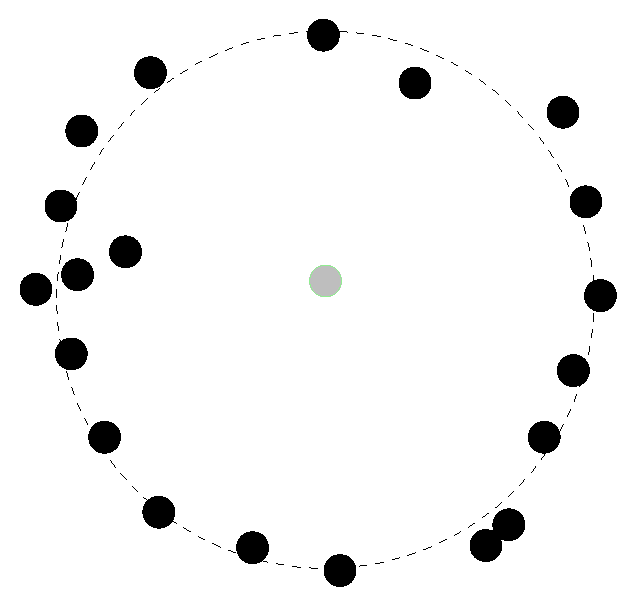
\includegraphics[width=.9\textwidth]{ES_0.eps}
%        \caption{$t$ = 0}
%      \end{figure}
%    \end{column}
%    \begin{column}{.33\textwidth}
%      \begin{figure}
%        \centering
%        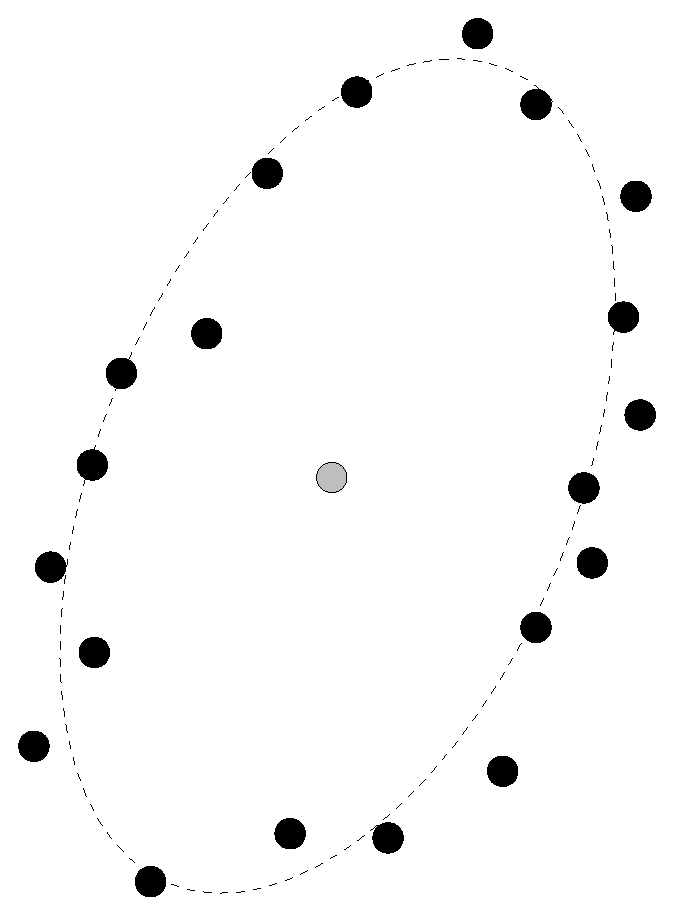
\includegraphics[width=.9\textwidth]{ES_10.eps}
%        \caption{$t$ = 10}
%      \end{figure}
%    \end{column}
%    \begin{column}{.33\textwidth}
%      \begin{figure}
%        \centering
%        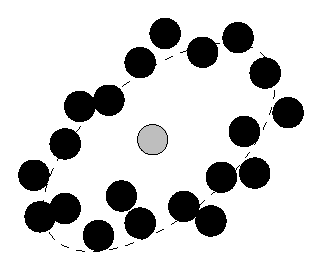
\includegraphics[width = .9\textwidth]{ES_20.eps}
%        \caption{$t$ = 20}
%      \end{figure}
%    \end{column}
%  \end{columns}
\end{frame}

